% Options for packages loaded elsewhere
% Options for packages loaded elsewhere
\PassOptionsToPackage{unicode}{hyperref}
\PassOptionsToPackage{hyphens}{url}
%
\documentclass[
  ignorenonframetext,
]{beamer}
\newif\ifbibliography
\usepackage{pgfpages}
\setbeamertemplate{caption}[numbered]
\setbeamertemplate{caption label separator}{: }
\setbeamercolor{caption name}{fg=normal text.fg}
\beamertemplatenavigationsymbolsempty
% remove section numbering
\setbeamertemplate{part page}{
  \centering
  \begin{beamercolorbox}[sep=16pt,center]{part title}
    \usebeamerfont{part title}\insertpart\par
  \end{beamercolorbox}
}
\setbeamertemplate{section page}{
  \centering
  \begin{beamercolorbox}[sep=12pt,center]{section title}
    \usebeamerfont{section title}\insertsection\par
  \end{beamercolorbox}
}
\setbeamertemplate{subsection page}{
  \centering
  \begin{beamercolorbox}[sep=8pt,center]{subsection title}
    \usebeamerfont{subsection title}\insertsubsection\par
  \end{beamercolorbox}
}
% Prevent slide breaks in the middle of a paragraph
\widowpenalties 1 10000
\raggedbottom
\AtBeginPart{
  \frame{\partpage}
}
\AtBeginSection{
  \ifbibliography
  \else
    \frame{\sectionpage}
  \fi
}
\AtBeginSubsection{
  \frame{\subsectionpage}
}
\usepackage{iftex}
\ifPDFTeX
  \usepackage[T1]{fontenc}
  \usepackage[utf8]{inputenc}
  \usepackage{textcomp} % provide euro and other symbols
\else % if luatex or xetex
  \usepackage{unicode-math} % this also loads fontspec
  \defaultfontfeatures{Scale=MatchLowercase}
  \defaultfontfeatures[\rmfamily]{Ligatures=TeX,Scale=1}
\fi
\usepackage{lmodern}

\usetheme[]{Madrid}
\usecolortheme[]{dolphin}
\ifPDFTeX\else
  % xetex/luatex font selection
\fi
% Use upquote if available, for straight quotes in verbatim environments
\IfFileExists{upquote.sty}{\usepackage{upquote}}{}
\IfFileExists{microtype.sty}{% use microtype if available
  \usepackage[]{microtype}
  \UseMicrotypeSet[protrusion]{basicmath} % disable protrusion for tt fonts
}{}
\makeatletter
\@ifundefined{KOMAClassName}{% if non-KOMA class
  \IfFileExists{parskip.sty}{%
    \usepackage{parskip}
  }{% else
    \setlength{\parindent}{0pt}
    \setlength{\parskip}{6pt plus 2pt minus 1pt}}
}{% if KOMA class
  \KOMAoptions{parskip=half}}
\makeatother


\usepackage{longtable,booktabs,array}
\usepackage{calc} % for calculating minipage widths
\usepackage{caption}
% Make caption package work with longtable
\makeatletter
\def\fnum@table{\tablename~\thetable}
\makeatother
\usepackage{graphicx}
\makeatletter
\newsavebox\pandoc@box
\newcommand*\pandocbounded[1]{% scales image to fit in text height/width
  \sbox\pandoc@box{#1}%
  \Gscale@div\@tempa{\textheight}{\dimexpr\ht\pandoc@box+\dp\pandoc@box\relax}%
  \Gscale@div\@tempb{\linewidth}{\wd\pandoc@box}%
  \ifdim\@tempb\p@<\@tempa\p@\let\@tempa\@tempb\fi% select the smaller of both
  \ifdim\@tempa\p@<\p@\scalebox{\@tempa}{\usebox\pandoc@box}%
  \else\usebox{\pandoc@box}%
  \fi%
}
% Set default figure placement to htbp
\def\fps@figure{htbp}
\makeatother


% definitions for citeproc citations
\NewDocumentCommand\citeproctext{}{}
\NewDocumentCommand\citeproc{mm}{%
  \begingroup\def\citeproctext{#2}\cite{#1}\endgroup}
\makeatletter
 % allow citations to break across lines
 \let\@cite@ofmt\@firstofone
 % avoid brackets around text for \cite:
 \def\@biblabel#1{}
 \def\@cite#1#2{{#1\if@tempswa , #2\fi}}
\makeatother
\newlength{\cslhangindent}
\setlength{\cslhangindent}{1.5em}
\newlength{\csllabelwidth}
\setlength{\csllabelwidth}{3em}
\newenvironment{CSLReferences}[2] % #1 hanging-indent, #2 entry-spacing
 {\begin{list}{}{%
  \setlength{\itemindent}{0pt}
  \setlength{\leftmargin}{0pt}
  \setlength{\parsep}{0pt}
  % turn on hanging indent if param 1 is 1
  \ifodd #1
   \setlength{\leftmargin}{\cslhangindent}
   \setlength{\itemindent}{-1\cslhangindent}
  \fi
  % set entry spacing
  \setlength{\itemsep}{#2\baselineskip}}}
 {\end{list}}
\usepackage{calc}
\newcommand{\CSLBlock}[1]{\hfill\break\parbox[t]{\linewidth}{\strut\ignorespaces#1\strut}}
\newcommand{\CSLLeftMargin}[1]{\parbox[t]{\csllabelwidth}{\strut#1\strut}}
\newcommand{\CSLRightInline}[1]{\parbox[t]{\linewidth - \csllabelwidth}{\strut#1\strut}}
\newcommand{\CSLIndent}[1]{\hspace{\cslhangindent}#1}



\setlength{\emergencystretch}{3em} % prevent overfull lines

\providecommand{\tightlist}{%
  \setlength{\itemsep}{0pt}\setlength{\parskip}{0pt}}



 


\usepackage{array}
\usepackage{ragged2e}
\usepackage{graphicx}
\usepackage{xcolor}
\usepackage{tikz}
\usepackage{setspace}
\setbeamercolor{frametitle}{bg=blue!60!black, fg=white}
\setbeamertemplate{frametitle}{
  \nointerlineskip
  \vskip-0.4cm
  \begin{beamercolorbox}[wd=\paperwidth,ht=1cm,dp=0.2cm,leftskip=0.3cm]{frametitle}
    \usebeamerfont{frametitle}\insertframetitle
  \end{beamercolorbox}
}
\setbeamertemplate{title page}{
    % --- Fondo blanco ---
    \setbeamercolor{background canvas}{bg=white}
    \centering

    % --- Franja azul sólo detrás del título ---
    \begin{tikzpicture}[remember picture,overlay]
     \fill[blue!50!black] ([yshift=-1cm]current page.north west) rectangle ([yshift=-3.2cm]current page.north east);
    \end{tikzpicture}

    % --- Título en blanco sobre fondo azul ---
    {\color{white}\Large\textbf{\inserttitle}\par}
    \vspace{0.4cm}
    % --- Autor, carrera y asesor ---
    {\large\textbf{Yulissa del Rocío Hernández Vázquez}\par}
    {\small Licenciatura en Matemáticas Aplicadas – FCFM UNACH\par}
    {\small Asesor: Yofre Hernán García Gómez\par}

    % --- Fecha ---
    \vspace{0.4cm}
    {\large Octubre 2025\par}

    % --- Logos centrados y más juntos debajo de la fecha ---
    \vspace{0.3cm}
    \begin{center}
    
\includegraphics[width=2cm]{logo.png}
    \hspace{0.1cm}
    
\includegraphics[width=1.7cm]{FCFM-logo.png}
    \end{center}
}
\makeatletter
\@ifpackageloaded{caption}{}{\usepackage{caption}}
\AtBeginDocument{%
\ifdefined\contentsname
  \renewcommand*\contentsname{Table of contents}
\else
  \newcommand\contentsname{Table of contents}
\fi
\ifdefined\listfigurename
  \renewcommand*\listfigurename{List of Figures}
\else
  \newcommand\listfigurename{List of Figures}
\fi
\ifdefined\listtablename
  \renewcommand*\listtablename{List of Tables}
\else
  \newcommand\listtablename{List of Tables}
\fi
\ifdefined\figurename
  \renewcommand*\figurename{Figure}
\else
  \newcommand\figurename{Figure}
\fi
\ifdefined\tablename
  \renewcommand*\tablename{Table}
\else
  \newcommand\tablename{Table}
\fi
}
\@ifpackageloaded{float}{}{\usepackage{float}}
\floatstyle{ruled}
\@ifundefined{c@chapter}{\newfloat{codelisting}{h}{lop}}{\newfloat{codelisting}{h}{lop}[chapter]}
\floatname{codelisting}{Listing}
\newcommand*\listoflistings{\listof{codelisting}{List of Listings}}
\makeatother
\makeatletter
\makeatother
\makeatletter
\@ifpackageloaded{caption}{}{\usepackage{caption}}
\@ifpackageloaded{subcaption}{}{\usepackage{subcaption}}
\makeatother

\usepackage{bookmark}
\IfFileExists{xurl.sty}{\usepackage{xurl}}{} % add URL line breaks if available
\urlstyle{same}
\hypersetup{
  pdftitle={Modelo de Optimización para Localización de Almacenes Preposicionados e Inventario Humanitario},
  pdfauthor={Yulissa del Rocío Hernández Vázquez},
  hidelinks,
  pdfcreator={LaTeX via pandoc}}


\title{Modelo de Optimización para Localización de Almacenes
Preposicionados e Inventario Humanitario}
\author{Yulissa del Rocío Hernández Vázquez}
\date{}

\begin{document}
\frame{\titlepage}


\begin{frame}{Contenido}
\phantomsection\label{contenido}
\begin{enumerate}
\tightlist
\item
  Introducción
\item
  Marco Teórico: Problema de Localización
\item
  Modelo de Inventarios EOQ Estocástico
\item
  Función Objetivo Integrada
\item
  Métricas de Desempeño
\item
  Aplicación en Chiapas
\item
  Escenarios Evaluados
\item
  Conclusiones
\end{enumerate}
\end{frame}

\begin{frame}{Introducción}
\phantomsection\label{introducciuxf3n}
\begin{columns}[T]
\begin{column}{0.6\linewidth}
\justifying
\setstretch{1.3}

La alta recurrencia de inundaciones y deslizamientos en \textbf{Chiapas}
afecta comunidades vulnerables. Este estudio busca optimizar la
respuesta humanitaria mediante la planificación previa, la ubicación
estratégica de almacenes y la gestión eficiente de recursos.

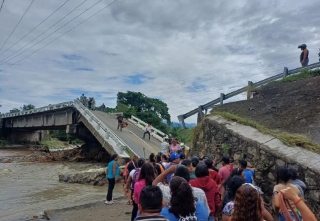
\includegraphics[width=0.55\linewidth,height=\textheight,keepaspectratio]{puente.png}
\end{column}

\begin{column}{0.4\linewidth}
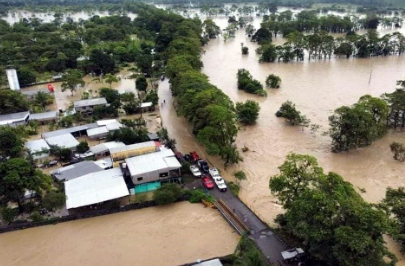
\includegraphics[width=1\linewidth,height=\textheight,keepaspectratio]{inundacion.png}
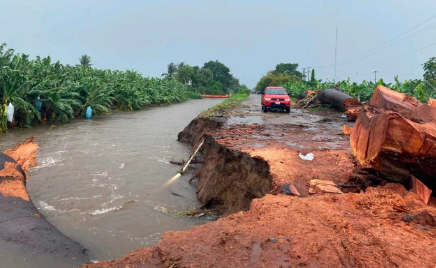
\includegraphics[width=1\linewidth,height=\textheight,keepaspectratio]{rio.png}
\end{column}
\end{columns}
\end{frame}

\begin{frame}{Objetivo Principal}
\phantomsection\label{objetivo-principal}
\begin{columns}[T]
\begin{column}{0.5\linewidth}
\justifying
\setstretch{1.3}

Desarrollar un modelo matemático integrado para optimizar la logística
humanitaria, determinando la ubicación estratégica de almacenes, niveles
de inventario y asignación de recursos que minimicen los costos
operativos durante emergencias.
\end{column}

\begin{column}{0.5\linewidth}
\centering

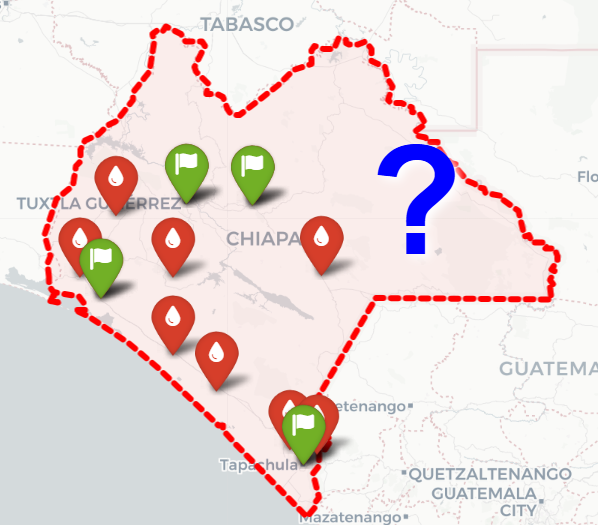
\includegraphics[width=0.8\linewidth,height=\textheight,keepaspectratio]{chiapas_almacen.png}
\end{column}
\end{columns}
\end{frame}

\begin{frame}{Marco Teórico: Problema de Localización}
\phantomsection\label{marco-teuxf3rico-problema-de-localizaciuxf3n}
Formulación Matemática

\textbf{Conjuntos:}

\begin{itemize}
\tightlist
\item
  \(I\): Localidades candidatas para almacenes
\item
  \(J\): Localidades demandantes (inundables)\\
\item
  \(P\): Productos humanitarios
\end{itemize}

\textbf{Variables de Decisión:}

\begin{itemize}
\tightlist
\item
  \(Y_i = 1\) si se instala almacén en \(i \in I\), \(0\) en otro caso
\item
  \(Y_{ij} = 1\) si localidad \(j\) es asignada a almacén \(i\), \(0\)
  en otro caso
\end{itemize}

\textbf{Parámetros Clave:}

\begin{itemize}
\tightlist
\item
  \(w_i\): Peso posicional (aptitud logística)
\item
  \(c_{ij}\): Costo de transporte
\item
  \(f_i\): Costo fijo de establecimiento
\end{itemize}
\end{frame}

\begin{frame}{Restricciones de Localización-Asignación}
\phantomsection\label{restricciones-de-localizaciuxf3n-asignaciuxf3n}
\textbf{Restricciones del Modelo}

Asignación Única: \[\sum_{i \in I} Y_{ij} = 1 \quad \forall j \in J\]

Factibilidad: \[Y_{ij} \leq Y_i \quad \forall i \in I, j \in J\]

Número de Almacenes: \[\sum_{i \in I} Y_i = A\]

Donde \(A\) es el número máximo de almacenes a instalar
\end{frame}

\begin{frame}{Modelo de Inventarios EOQ con demanda Estocástica}
\phantomsection\label{modelo-de-inventarios-eoq-con-demanda-estocuxe1stica}
\begin{columns}[T]
\begin{column}{0.5\linewidth}
\textbf{Cantidad Económica de Pedido:} \[Q^* = \sqrt{\frac{2DS}{H}}\]

\textbf{Componentes:}

\begin{itemize}
\tightlist
\item
  \(D\): Demanda anual del producto
\item
  \(S\): Costo de ordenar por pedido
\item
  \(H\): Costo de mantener inventario
\end{itemize}
\end{column}

\begin{column}{0.5\linewidth}
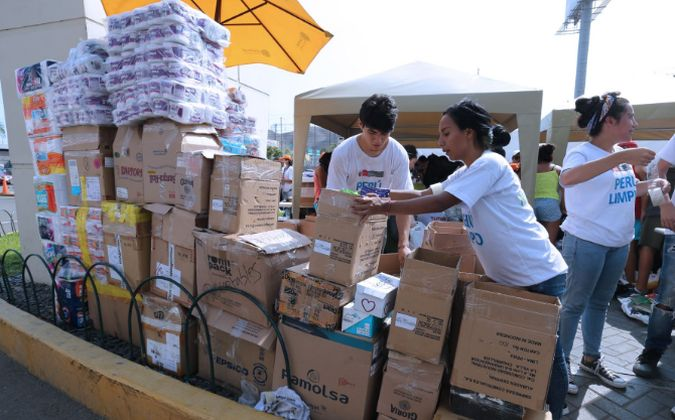
\includegraphics[width=0.85\linewidth,height=\textheight,keepaspectratio]{ayuda.png}
\end{column}
\end{columns}

\textbf{Adaptación para Contexto Humanitario}

\begin{itemize}
\tightlist
\item
  \textbf{Demanda estocástica} por incertidumbre en afectación
\item
  \textbf{Horizonte temporal} ajustado a emergencias
\item
  \textbf{Múltiples productos} con características diferentes
\end{itemize}
\end{frame}

\begin{frame}{Inventario de Seguridad y Punto de Reorden}
\phantomsection\label{inventario-de-seguridad-y-punto-de-reorden}
\begin{columns}[T]
\begin{column}{0.5\linewidth}
\textbf{Inventario de Seguridad:}
\[SS = Z_{\alpha} \cdot \sigma_d \cdot \sqrt{L}\]

\textbf{Punto de Reorden:} \[R = d \cdot L + SS\]
\end{column}

\begin{column}{0.5\linewidth}
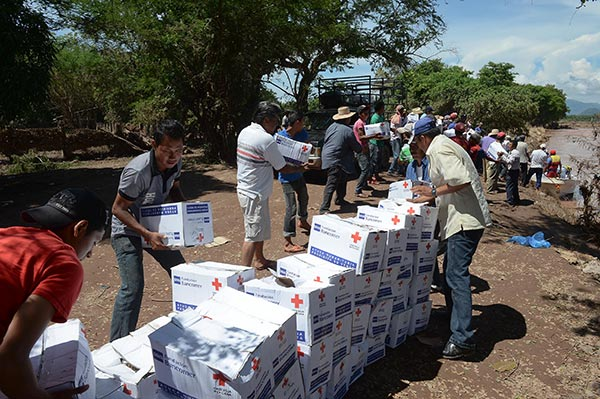
\includegraphics[width=0.85\linewidth,height=\textheight,keepaspectratio]{ayu.png}
\end{column}
\end{columns}

\textbf{donde:}

\begin{itemize}
\tightlist
\item
  \(Z_{\alpha}\): Valor Z para nivel de servicio \(\alpha\) (95\%)
\item
  \(\sigma_d\): Desviación estándar de demanda diaria
\item
  \(L\): Tiempo de entrega en días
\item
  \(d\): Demanda diaria promedio
\end{itemize}
\end{frame}

\begin{frame}{Función de Pérdida Normal}
\phantomsection\label{funciuxf3n-de-puxe9rdida-normal}
Para estimar el riesgo de escasez, usamos la función de pérdida asociada
a la distribución normal:

\begin{columns}[T]
\begin{column}{0.4\linewidth}
\[E[Z] = \phi(Z) - Z(1 - \Phi(Z))\]
\end{column}

\begin{column}{0.6\linewidth}
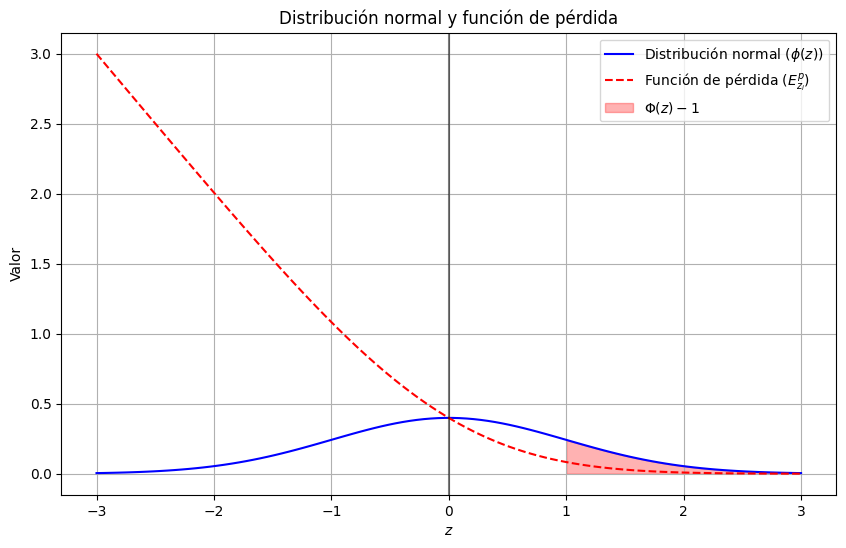
\includegraphics[width=1\linewidth,height=\textheight,keepaspectratio]{funcion_perdida.png}
\end{column}
\end{columns}

\textbf{Aplicación en Fill Rate:}

\begin{itemize}
\tightlist
\item
  \textbf{Fill Rate} = Proporción de demanda satisfecha
\item
  \textbf{Relación directa} con nivel de servicio
\item
  \textbf{Base para cálculo} de costos por escasez
\end{itemize}
\end{frame}

\begin{frame}{Función Objetivo}
\phantomsection\label{funciuxf3n-objetivo}
\textbf{Minimización de Costos Totales}

\[
\min Z =
\sum_{i \in I} f_i Y_i +
\sum_{i \in I} \sum_{j \in J} w_i c_{ij} Y_{ij} +
\sum_{i \in I} \sum_{p \in P} TC_{ip}
\]

Esta función minimiza el \textbf{costo total del sistema logístico
humanitario}, combinando decisiones de \textbf{localización, transporte
e inventario}.
\end{frame}

\begin{frame}{Componentes del Costo de Inventario}
\phantomsection\label{componentes-del-costo-de-inventario}
\[
TC_{ip} =
{\color{blue}\frac{C^{op}_i D^p_j}{Q^p_{ij}} +
C^{sp}_i \left(\frac{Q^p_{ij}}{2} + SS\right) +
C^p_i D^p_j} {\color{red}+
\frac{D^p_j}{Q^p_{ij}} (C^f_i + \sigma_d E[Z] B)}
\]

\begin{itemize}
\tightlist
\item
  \({\textcolor{blue}{\textbf{Costo de pedido o preparación}}}\): se
  reduce al aumentar la cantidad pedida.\\
\item
  \({\textcolor{blue}{\textbf{Costo de mantenimiento o almacenamiento}}}\):
  considerando el inventario promedio y la seguridad \(SS\).\\
\item
  \({\textcolor{blue}{\textbf{Costo de adquisición}}}\): asociado a la
  demanda esperada \(D^p_j\) del producto \(p\).\\
\item
  \({\textcolor{red}{\textbf{Costo esperado de faltante}}}\): incorpora
  la variabilidad de la demanda \(\sigma_d\) y el costo unitario de
  escasez \(B\).
\end{itemize}
\end{frame}

\begin{frame}{Peso Posicional}
\phantomsection\label{peso-posicional}
\begin{columns}[T]
\begin{column}{0.5\linewidth}
\textbf{Multicriterio para Selección}

Componentes del Peso Posicional \(w_i\):

\begin{itemize}
\tightlist
\item
  \textbf{Accesibilidad por carretera}
\item
  \textbf{Existencia de servicios básicos}
\item
  \textbf{Infraestructura disponible}
\end{itemize}
\end{column}

\begin{column}{0.5\linewidth}

\includegraphics[width=0.85\linewidth,height=\textheight,keepaspectratio]{peso.png}
\end{column}
\end{columns}

\textbf{Objetivo:}

Priorizar localidades con \textbf{mayor capacidad logística} y
\textbf{menor vulnerabilidad estructural}
\end{frame}

\begin{frame}{Métricas de Desempeño}
\phantomsection\label{muxe9tricas-de-desempeuxf1o}
\textbf{Fill Rate del Sistema:}
\[FR_{sistema} = \frac{\sum_{i \in I} \sum_{p \in P} D_{ip} \cdot FR_{ip}}{\sum_{i \in I} \sum_{p \in P} D_{ip}}\]

\textbf{Costo Total por Persona Atendida:}

\[Costo_{pe} = \frac{Costo_{t}}{Poblacion_{a}}\]

\textbf{Tiempo Promedio de Respuesta:}
\[T_{respuesta} = \frac{\sum_{i \in I} \sum_{j \in J} t_{ij} \cdot Y_{ij}}{\sum_{i \in I} \sum_{j \in J} Y_{ij}}\]

Donde:

\begin{itemize}
\tightlist
\item
  \(t_{ij}\) : tiempo de transporte (horas) desde el almacén \(𝑖\) hasta
  la zona afectada \(𝑗\).
\end{itemize}
\end{frame}

\begin{frame}{Aplicación en Chiapas}
\phantomsection\label{aplicaciuxf3n-en-chiapas}
\begin{columns}[T]
\begin{column}{0.6\linewidth}
\justifying

\textbf{Características de Chiapas:}

\begin{itemize}
\tightlist
\item
  \textbf{Alta vulnerabilidad} a inundaciones y deslizamientos
\item
  \textbf{Topografía compleja} que afecta accesibilidad
\item
  \textbf{Población dispersa} en comunidades rurales
\item
  \textbf{Recursos limitados} para logística humanitaria
\end{itemize}

\textbf{Productos Humanitarios Considerados:}

\begin{itemize}
\tightlist
\item
  Agua potable (2 litros/persona/día)
\item
  Alimentos no perecederos
\item
  Kits de medicamentos básicos
\item
  Ropa y cobijas
\item
  Artículos de higiene personal
\end{itemize}
\end{column}

\begin{column}{0.4\linewidth}
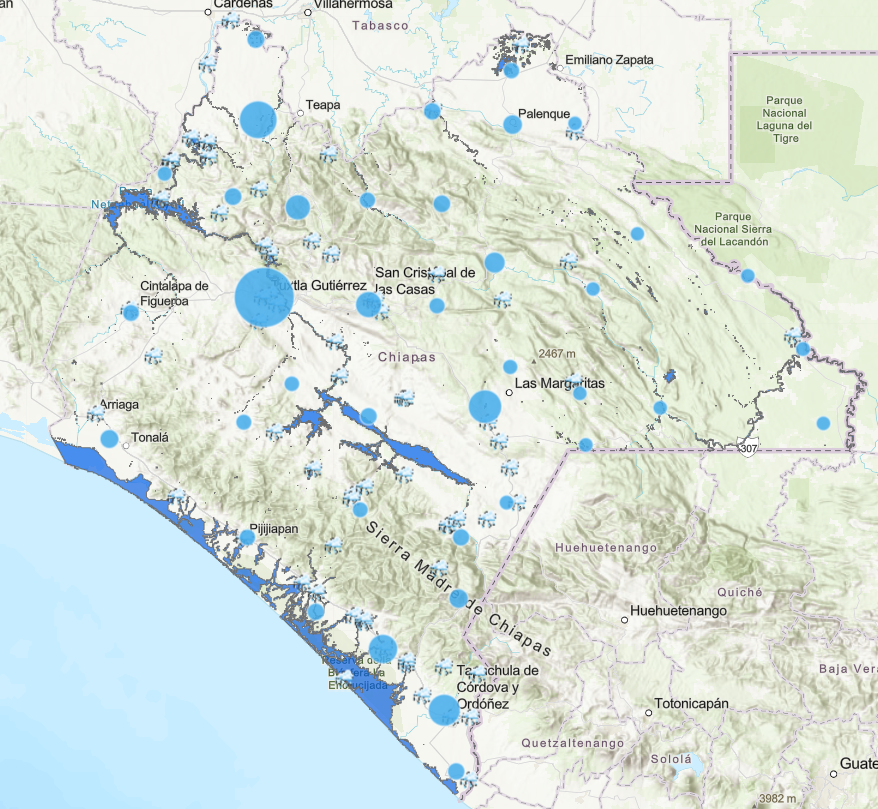
\includegraphics[width=0.8\linewidth,height=\textheight,keepaspectratio]{chiapas.png}
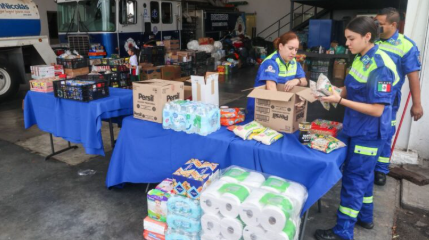
\includegraphics[width=1\linewidth,height=\textheight,keepaspectratio]{productos.png}
\end{column}
\end{columns}
\end{frame}

\begin{frame}{Cálculo del Peso Posicional --- Caso Chiapas}
\phantomsection\label{cuxe1lculo-del-peso-posicional-caso-chiapas}
El peso posicional \(w_j\) integra cinco dimensiones logísticas de
relevancia humanitaria, cada una con ponderación del 20 \%. Se
normalizaron todas las variables en el rango \([0,1]\):

\[w_i = 0.20 (Diconsa_i +  AccesoVial_i +  Escuelas_i +  Servicios_i + Poblacion_i)\]

\textbf{Top 5 localidades con mayor potencial logístico (Cacahoatán):}

\begin{longtable}[]{@{}clc@{}}
\toprule\noalign{}
\textbf{\#} & \textbf{Localidad} & \textbf{Peso} \\
\midrule\noalign{}
\endhead
1 & Salvador Urbina & \textbf{1.000} \\
2 & Faja de Oro & \textbf{0.983} \\
3 & Cacahoatán & 0.849 \\
4 & Rosario Ixtal & 0.749 \\
5 & Mixcum & 0.657 \\
\bottomrule\noalign{}
\end{longtable}
\end{frame}

\begin{frame}{Escenarios Evaluados --- Cacahoatán}
\phantomsection\label{escenarios-evaluados-cacahoatuxe1n}
\textbf{Objetivo:} Analizar la sensibilidad del modelo ante
restricciones espaciales.

🔹 Escenario A: Sin radio de afectación

\begin{itemize}
\tightlist
\item
  Se evaluaron \textbf{2 almacenes candidatos}.\\
\item
  El modelo seleccionó \textbf{1 almacén óptimo} que cubre las 4
  localidades.\\
\item
  Solución \textbf{eficiente en costo} y \textbf{plena cobertura} del
  territorio.
\end{itemize}

\begin{columns}[T]
\begin{column}{0.6\linewidth}
\begin{longtable}[]{@{}ll@{}}
\toprule\noalign{}
Indicador & Resultado \\
\midrule\noalign{}
\endhead
Cobertura & 100 \% \\
Población atendida & 7,407 personas \\
Localidades cubiertas & 4 \\
Fill rate promedio & 100 \% \\
Costo total anual & \$195,459,693 MXN \\
\bottomrule\noalign{}
\end{longtable}
\end{column}

\begin{column}{0.4\linewidth}
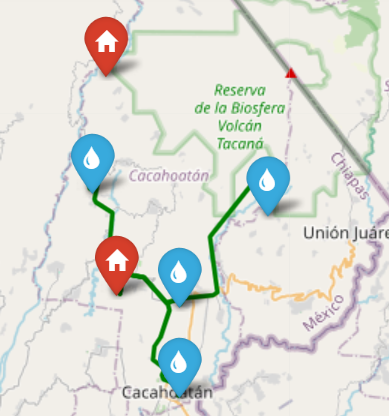
\includegraphics[width=0.8\linewidth,height=\textheight,keepaspectratio]{almacen.png}
\end{column}
\end{columns}
\end{frame}

\begin{frame}{Continuación Escenarios Evaluados --- Cacahoatán}
\phantomsection\label{continuaciuxf3n-escenarios-evaluados-cacahoatuxe1n}
\begin{columns}[T]
\begin{column}{0.5\linewidth}
🔹 Escenario B: Con radio de afectación \(r = 5\) km

\begin{itemize}
\tightlist
\item
  El \textbf{almacén 1} queda \textbf{dentro del radio de influencia}
  del segundo.\\
\item
  El modelo selecciona el \textbf{almacén 2} como óptimo.\\
\item
  Se mantiene \textbf{cobertura total}, pero con \textbf{mayor
  eficiencia espacial}.
\end{itemize}
\end{column}

\begin{column}{0.5\linewidth}
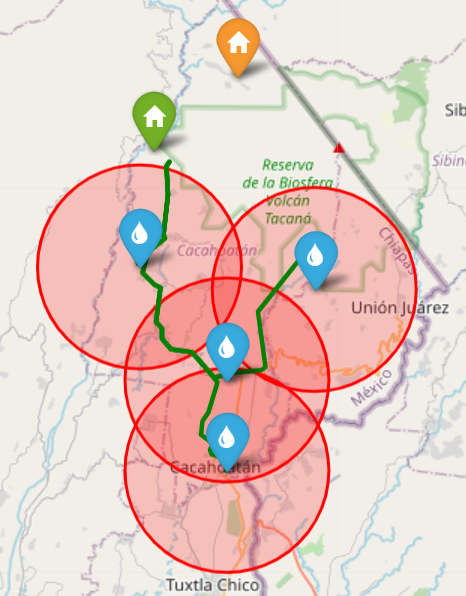
\includegraphics[width=0.7\linewidth,height=\textheight,keepaspectratio]{radio.png}
\end{column}
\end{columns}

La restricción geográfica redefine la ubicación óptima, evidenciando la
importancia de integrar criterios espaciales en la localización
humanitaria.
\end{frame}

\begin{frame}{Análisis de Sensibilidad}
\phantomsection\label{anuxe1lisis-de-sensibilidad}
\textbf{Factor de Afectación:}

\begin{itemize}
\tightlist
\item
  Escenario base: \textbf{30\%} de población afectada
\item
  Análisis de sensibilidad: \textbf{20\% - 50\%}
\end{itemize}

\textbf{Nivel de Servicio:}

\begin{itemize}
\tightlist
\item
  Objetivo principal: \textbf{95\%} fill rate
\item
  Variación: \textbf{90\% - 99\%}
\end{itemize}

\textbf{Número de Almacenes:}

\begin{itemize}
\tightlist
\item
  Rango evaluado: \textbf{1 - 4 almacenes}
\item
  Trade-off: \textbf{Costo vs.~Cobertura}
\end{itemize}
\end{frame}

\begin{frame}{Conclusiones}
\phantomsection\label{conclusiones}
Hallazgos Principales

\textbf{Efectividad del Modelo:}

\begin{itemize}
\tightlist
\item
  \textbf{Integración exitosa} de localización e inventario
\item
  \textbf{Balance óptimo} entre costos y nivel de servicio
\item
  \textbf{Aplicabilidad práctica} en contextos reales
\end{itemize}

\textbf{Contribuciones:}

\begin{itemize}
\tightlist
\item
  \textbf{Marco decisiona}l para planificación pre-desastre
\item
  \textbf{Herramienta cuantitativa} para agencias humanitarias
\item
  \textbf{Base metodológica} replicable en otros municipios
\end{itemize}

\vspace{1em}

\begin{block}{}
\centering
\large
\textit{
“Chiapas y Veracruz enfrentan desastres distintos, pero comparten una misma esperanza:  
que la preparación salve más vidas que la reacción,  
porque entre montañas o planicies, el agua no distingue fronteras,  
pero la prevención sí puede marcar la diferencia.”
}
\end{block}
\end{frame}

\begin{frame}{Recomendaciones para Cacahoatán}
\phantomsection\label{recomendaciones-para-cacahoatuxe1n}
\begin{itemize}
\tightlist
\item
  \textbf{Implementar configuración} de 2 almacenes
\item
  \textbf{Mantener inventarios} según cálculo EOQ con demanda
  Estocástica
\item
  \textbf{Monitorear continuamente} factores de riesgo
\end{itemize}
\end{frame}

\begin{frame}{Referencias}
\phantomsection\label{referencias}
\phantomsection\label{refs}
\begin{CSLReferences}{1}{0}
\bibitem[\citeproctext]{ref-BarojasPayan2021}
Barojas-Payán, E., D. Sánchez-Partida, et al. 2021. {``Optimization
Model to Locate Pre-Positioned Warehouses.''} In \emph{Disaster Risk
Reduction in Mexico}, edited by D. Sánchez-Partida, 169--98. Springer.
\url{https://doi.org/10.1007/978-3-030-67295-9_8}.

\bibitem[\citeproctext]{ref-ArcGIS2024}
Esri México. 2024. {``Visor de Infraestructura y Riesgos de
Desastres.''}
\url{https://atlsrgochis.maps.arcgis.com/apps/webappviewer/index.html?id=e0e724ad2bb8423894b0cebd1f27a7d5}.

\bibitem[\citeproctext]{ref-INEGI2024}
INEGI. 2024. {``Bases de Datos y Visor Geoespacial.''}
\url{https://www.inegi.org.mx/app/mapa/denue/}.

\bibitem[\citeproctext]{ref-SEP2024}
Secretaría de Educación Pública (SEP). 2024. {``Principales Cifras Del
Sistema Educativo Nacional.''}
\url{https://www.planeacion.sep.gob.mx/principalescifras/}.

\bibitem[\citeproctext]{ref-Taha2016}
Taha, Hamdy A. 2016. \emph{Operations Research: An Introduction}. 10th
ed. Pearson.

\end{CSLReferences}
\end{frame}




\end{document}
